
\subsection{CODEC driver}

\begin{frame}[fragile]{CODEC driver}
  The CODEC driver registers a \code{struct snd_soc_component_driver}.
  Before v4.17, it was \code{struct snd_soc_codec_driver}.
  Also registers a \code{struct snd_soc_dai_driver}

  \begin{block}{\code{include/sound/soc.h}}
    \fontsize{9}{9}\selectfont
    \begin{minted}{c}
int snd_soc_register_component(struct device *dev,
                 const struct snd_soc_component_driver *component_driver,
                 struct snd_soc_dai_driver *dai_drv, int num_dai);
int devm_snd_soc_register_component(struct device *dev,
                 const struct snd_soc_component_driver *component_driver,
                 struct snd_soc_dai_driver *dai_drv, int num_dai);
    \end{minted}
  \end{block}
\end{frame}

\begin{frame}[fragile]{\code{snd_soc_component_driver}}
  \begin{block}{\code{include/sound/soc-component.h}}
    \fontsize{9}{9}\selectfont
    \begin{minted}{c}
struct snd_soc_component_driver {
        const char *name;

        /* Default control and setup, added after probe() is run */
        const struct snd_kcontrol_new *controls;
        unsigned int num_controls;
        const struct snd_soc_dapm_widget *dapm_widgets;
        unsigned int num_dapm_widgets;
        const struct snd_soc_dapm_route *dapm_routes;
        unsigned int num_dapm_routes;

        int (*probe)(struct snd_soc_component *component);
        void (*remove)(struct snd_soc_component *component);
        int (*suspend)(struct snd_soc_component *component);
        int (*resume)(struct snd_soc_component *component);

    [...]
    \end{minted}
  \end{block}
\end{frame}

\begin{frame}{\code{snd_soc_component_driver}}
  \begin{itemize}
  \item \code{struct snd_kcontrol_new *controls} is an array of
    controls (volume, mixing, muxing, switches) available on the
    CODEC.
  \item \code{struct snd_soc_dapm_widget *dapm_widgets} is an array of
    power management controls so ASoC can power down the routes that
    are not currently used.
  \item \code{struct snd_soc_dapm_route *dapm_routes} is an array
    describing those routes.
  \end{itemize}
\end{frame}

\begin{frame}[fragile]{\code{snd_soc_component_driver}}
  \begin{block}{\code{include/sound/soc-component.h}}
    \fontsize{9}{9}\selectfont
    \begin{minted}{c}
        /* component wide operations */
        int (*set_sysclk)(struct snd_soc_component *component,
                          int clk_id, int source, unsigned int freq, int dir);
        int (*set_pll)(struct snd_soc_component *component, int pll_id,
                       int source, unsigned int freq_in, unsigned int freq_out);
        [...]
        int (*hw_params)(struct snd_soc_component *component,
                         struct snd_pcm_substream *substream,
                         struct snd_pcm_hw_params *params);
        [...]
}
    \end{minted}
  \end{block}
\end{frame}

\begin{frame}{\code{snd_soc_component_driver}}
  \begin{itemize}
  \item \code{set_sysclk} allows setting the input clock of the
    component.
  \item \code{set_pll} allows setting the PLLs, this is mostly useful
    when the component is the clock producer.
  \item \code{hw_params} is a callback called on PCM stream setup.
    When called, all the parameters of the stream are known so it is
    possible to configure the component to handle the stream
    correctly.
  \item Those are mostly not used, the DAI specific callbacks are used
    instead.
  \end{itemize}
\end{frame}

\begin{frame}[fragile]{\code{snd_soc_dai_driver}}
  \begin{block}{\code{include/sound/soc-dai.h}}
    \fontsize{8}{8}\selectfont
    \begin{minted}{c}
/*
 * Digital Audio Interface Driver.
 *
 * Describes the Digital Audio Interface in terms of its ALSA, DAI and AC97
 * operations and capabilities. Codec and platform drivers will register this
 * structure for every DAI they have.
 *
 * This structure covers the clocking, formating and ALSA operations for each
 * interface.
 */
struct snd_soc_dai_driver {
        /* DAI description */
        const char *name;
        [...]

        /* ops */
        const struct snd_soc_dai_ops *ops;
        const struct snd_soc_cdai_ops *cops;

        /* DAI capabilities */
        struct snd_soc_pcm_stream capture;
        struct snd_soc_pcm_stream playback;
        [...]
};
    \end{minted}
  \end{block}
\end{frame}

\begin{frame}[fragile]{\code{snd_soc_pcm_stream}}
  \begin{block}{\code{include/sound/soc.h}}
    \fontsize{9}{9}\selectfont
    \begin{minted}{c}
/* SoC PCM stream information */
struct snd_soc_pcm_stream {
        const char *stream_name;
        u64 formats;                       /* SNDRV_PCM_FMTBIT_* */
        unsigned int rates;                /* SNDRV_PCM_RATE_* */
        unsigned int rate_min;             /* min rate */
        unsigned int rate_max;             /* max rate */
        unsigned int channels_min;         /* min channels */
        unsigned int channels_max;         /* max channels */
        unsigned int sig_bits;             /* number of bits of content */
};
    \end{minted}
  \end{block}
\end{frame}

\begin{frame}[fragile]{PCM5102}
  \begin{center}
  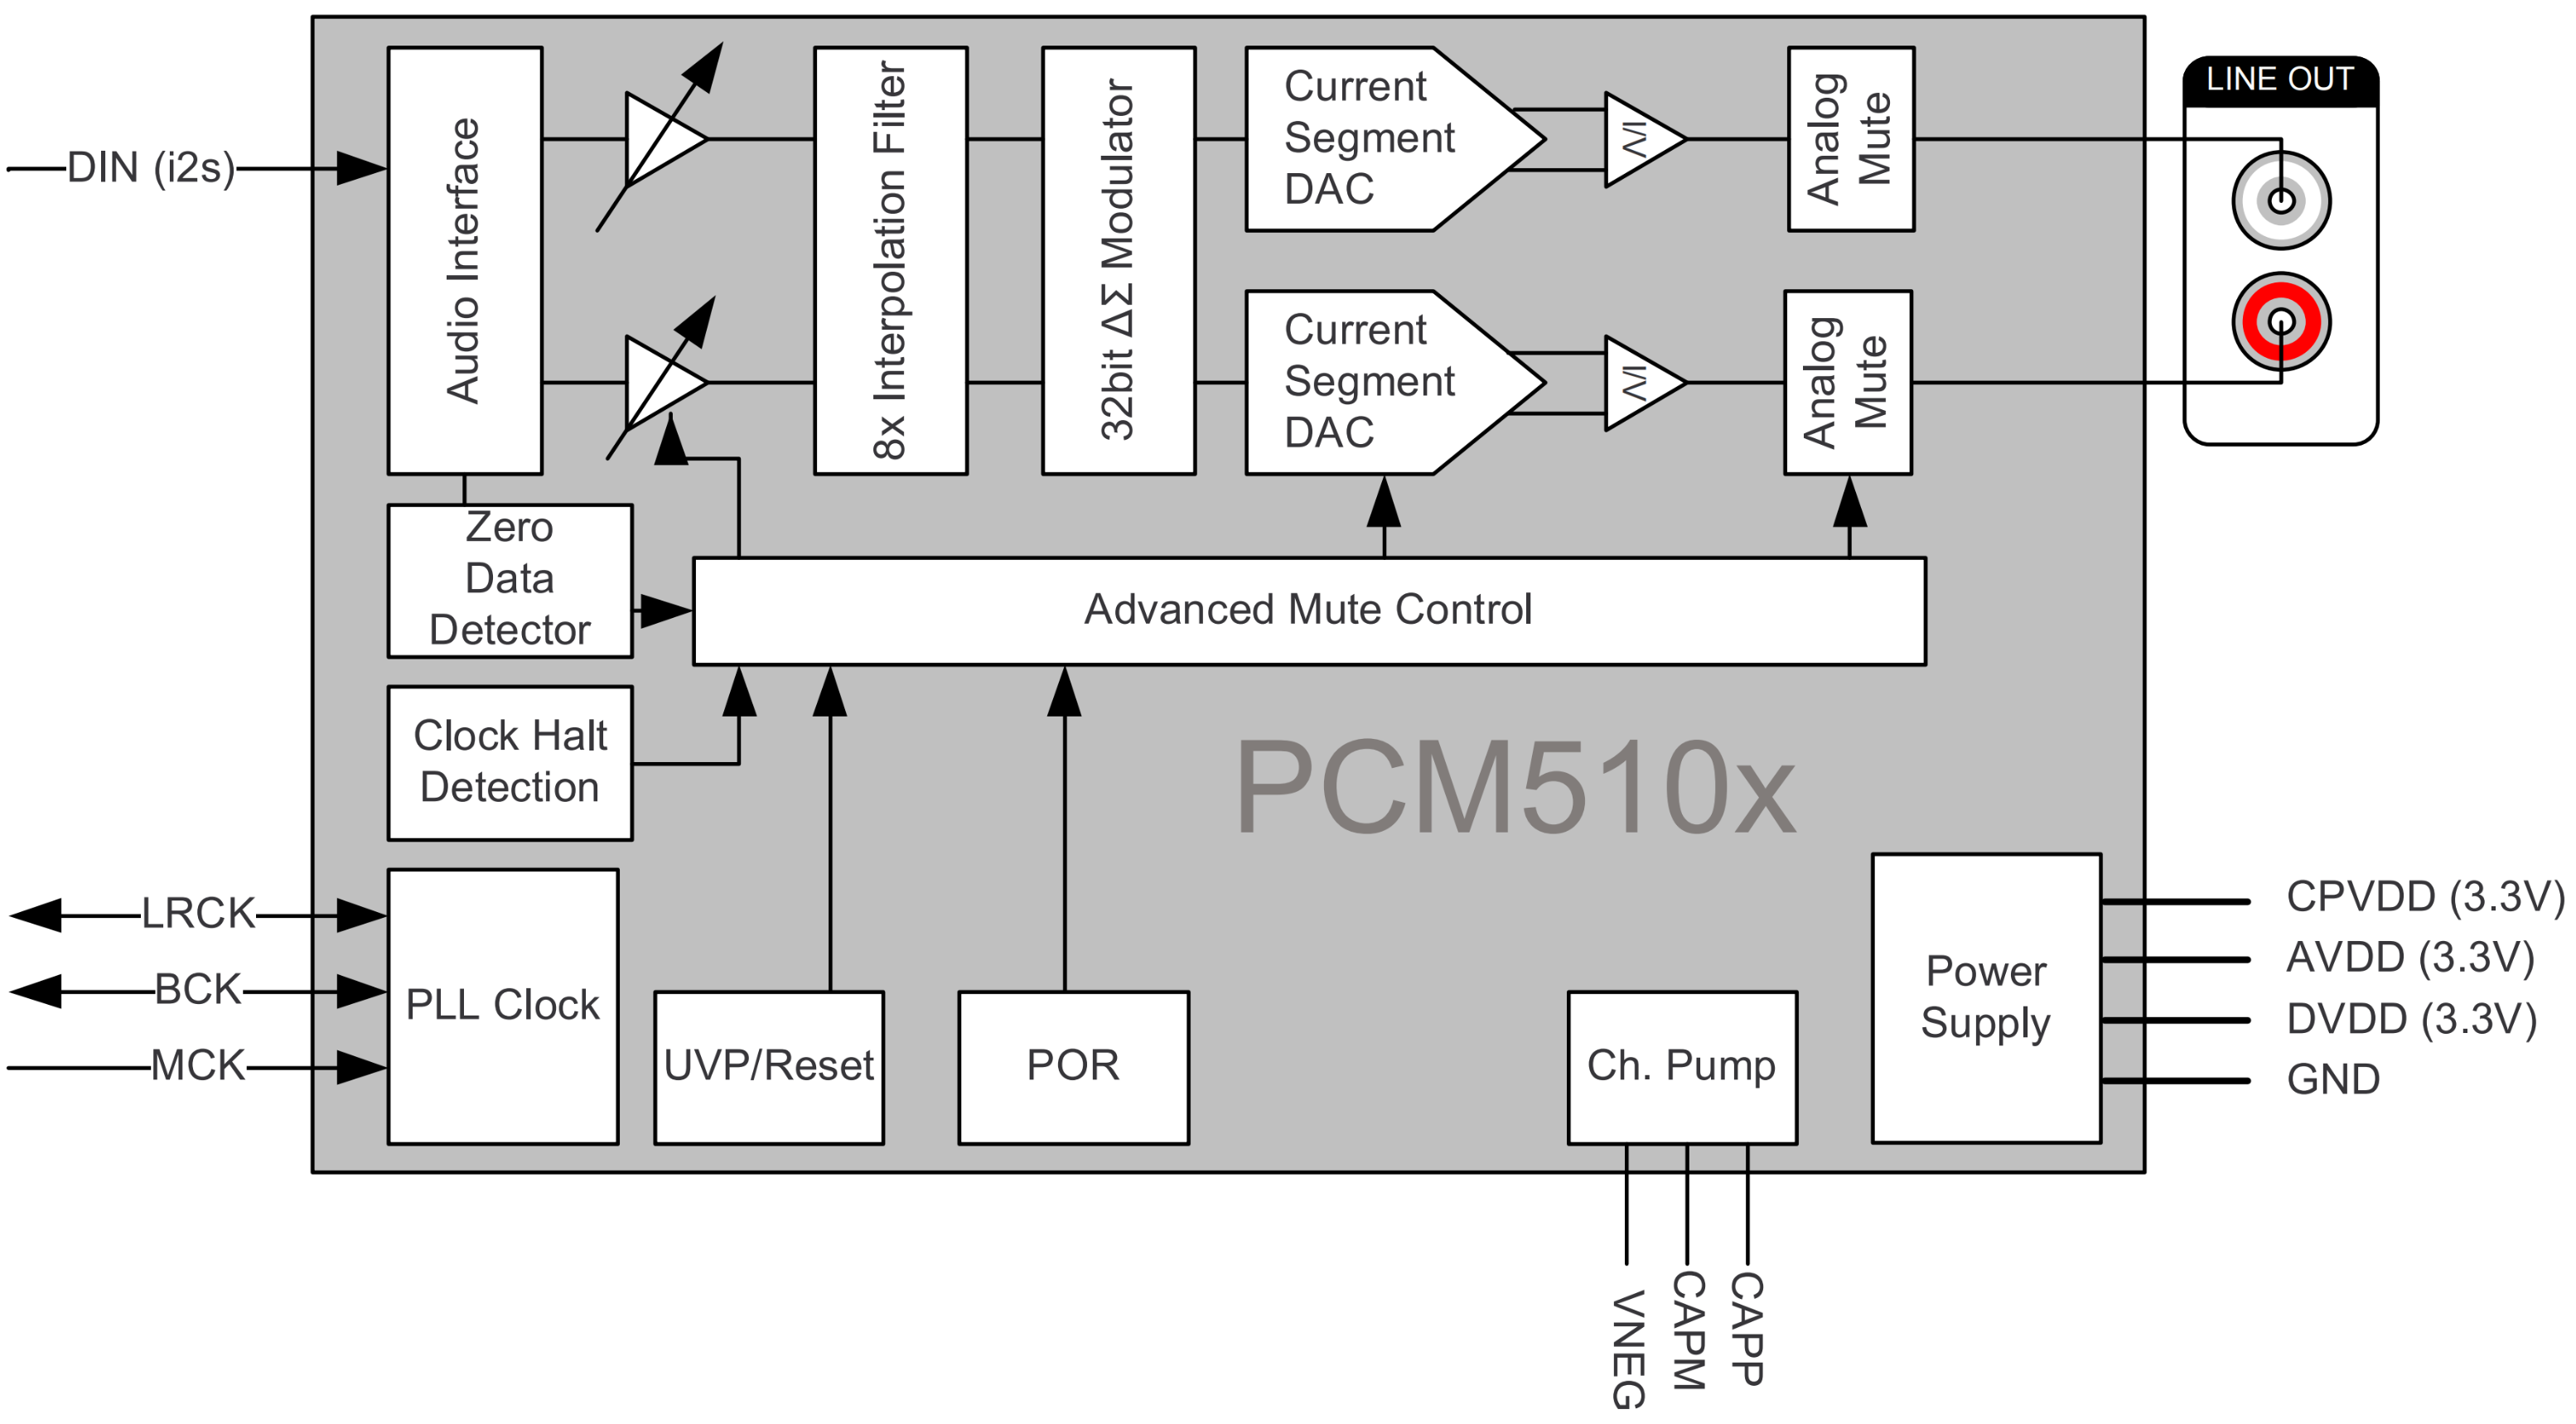
\includegraphics[width=0.9\textwidth]{slides/audio-asoc-codec/pcm510x.png}
  \end{center}
\end{frame}

\begin{frame}[fragile]{\code{pcm5102a.c}}
  \begin{block}{\code{sound/soc/codecs/pcm5102a.c}}
    \fontsize{8}{8}\selectfont
    \begin{minted}{c}
static struct snd_soc_dai_driver pcm5102a_dai = {
        .name = "pcm5102a-hifi",
        .playback = {
                .channels_min = 2,
                .channels_max = 2,
                .rates = SNDRV_PCM_RATE_8000_384000,
                .formats = SNDRV_PCM_FMTBIT_S16_LE |
                           SNDRV_PCM_FMTBIT_S24_LE |
                           SNDRV_PCM_FMTBIT_S32_LE
        },
};

static struct snd_soc_component_driver soc_component_dev_pcm5102a = {
        .idle_bias_on                = 1,
        .use_pmdown_time             = 1,
        .endianness                  = 1,
};

static int pcm5102a_probe(struct platform_device *pdev)
{
        return devm_snd_soc_register_component(&pdev->dev, &soc_component_dev_pcm5102a,
                        &pcm5102a_dai, 1);
}
    \end{minted}
  \end{block}
\end{frame}

\begin{frame}[fragile]{PCM3008}
  \begin{center}
  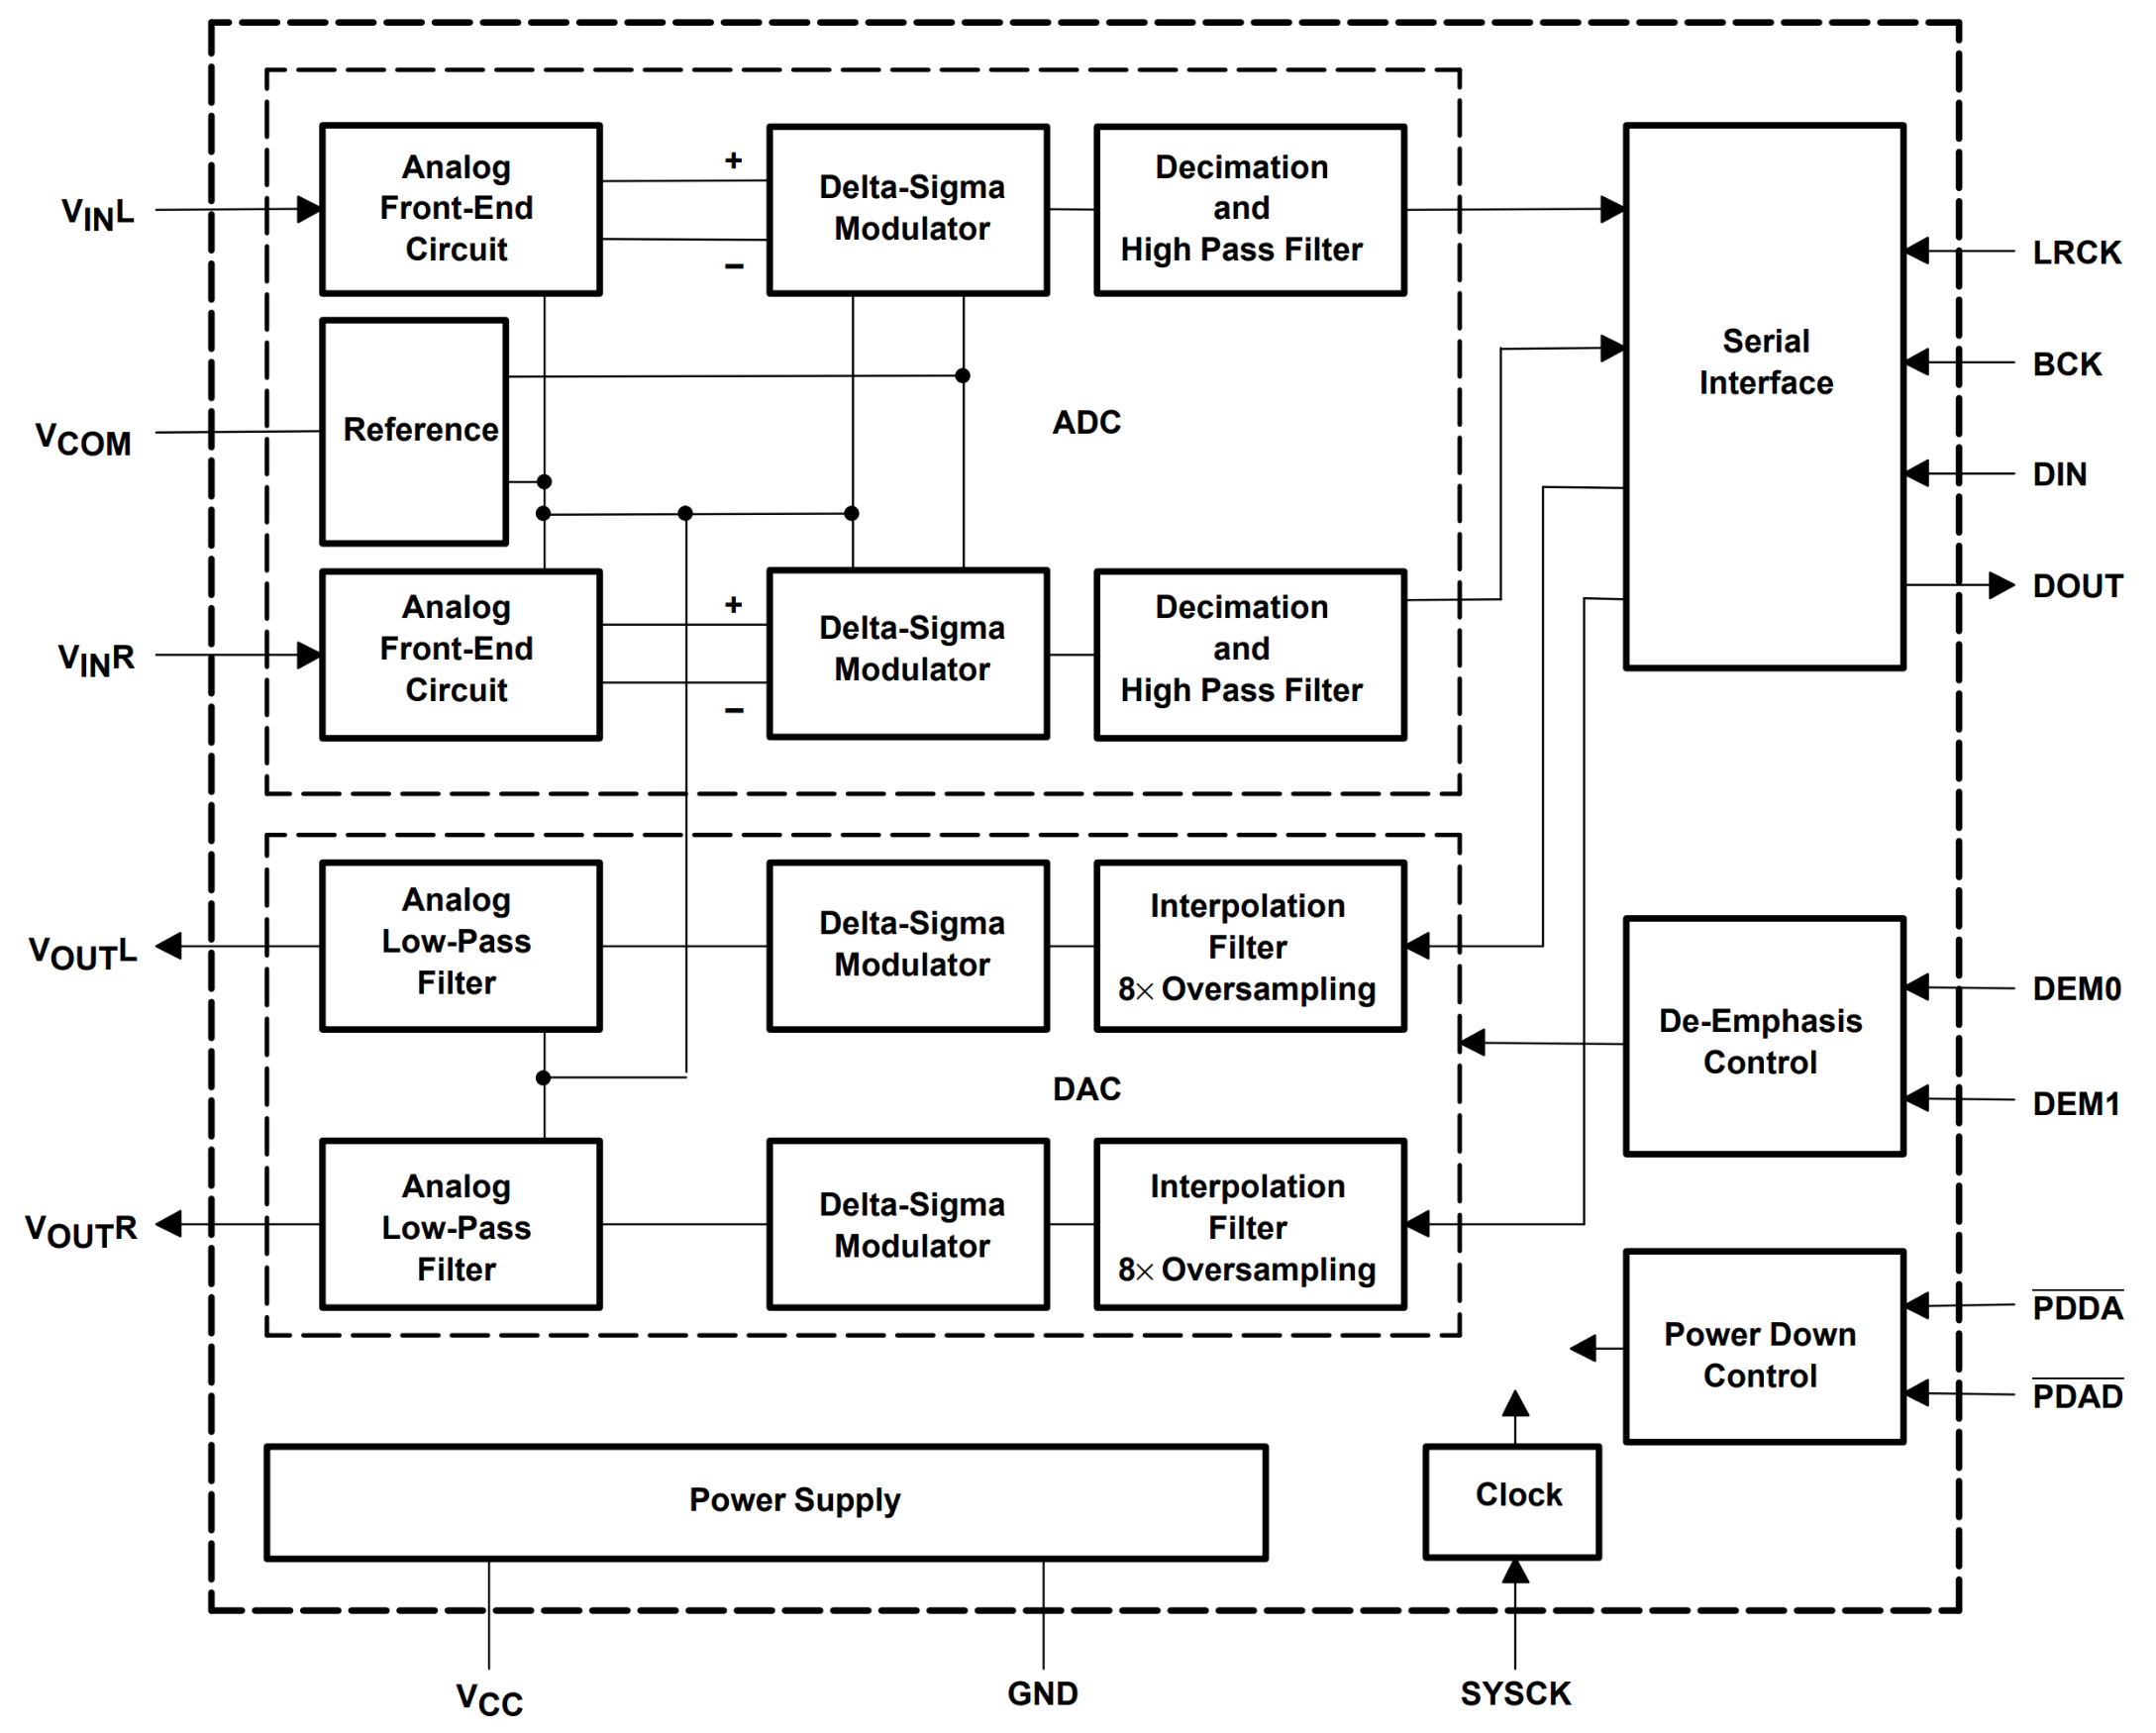
\includegraphics[width=0.7\textwidth]{slides/audio-asoc-codec/pcm3008.png}
  \end{center}
\end{frame}

\begin{frame}[fragile]{\code{pcm3008.c}}
  \begin{block}{\code{sound/soc/codecs/pcm3008.c}}
    \fontsize{9}{9}\selectfont
    \begin{minted}{c}
#define PCM3008_RATES (SNDRV_PCM_RATE_32000 | SNDRV_PCM_RATE_44100 |        \
                       SNDRV_PCM_RATE_48000)

static struct snd_soc_dai_driver pcm3008_dai = {
        .name = "pcm3008-hifi",
        .playback = {
                .stream_name = "PCM3008 Playback",
                .channels_min = 1,
                .channels_max = 2,
                .rates = PCM3008_RATES,
                .formats = SNDRV_PCM_FMTBIT_S16_LE,
        },
        .capture = {
                .stream_name = "PCM3008 Capture",
                .channels_min = 1,
                .channels_max = 2,
                .rates = PCM3008_RATES,
                .formats = SNDRV_PCM_FMTBIT_S16_LE,
        },
};
    \end{minted}
  \end{block}
\end{frame}

\begin{frame}[fragile]{\code{pcm3008.c}}
  \begin{block}{\code{sound/soc/codecs/pcm3008.c}}
    \fontsize{9}{9}\selectfont
    \begin{minted}{c}
static const struct snd_soc_component_driver soc_component_dev_pcm3008 = {
        .dapm_widgets           = pcm3008_dapm_widgets,
        .num_dapm_widgets       = ARRAY_SIZE(pcm3008_dapm_widgets),
        .dapm_routes            = pcm3008_dapm_routes,
        .num_dapm_routes        = ARRAY_SIZE(pcm3008_dapm_routes),
        .idle_bias_on           = 1,
        .use_pmdown_time        = 1,
        .endianness             = 1,
};

static int pcm3008_codec_probe(struct platform_device *pdev)
{
        [...]

        return devm_snd_soc_register_component(&pdev->dev,
                        &soc_component_dev_pcm3008, &pcm3008_dai, 1);
}
    \end{minted}
  \end{block}
\end{frame}

\begin{frame}[fragile]{\code{pcm3008.c}}
  \begin{block}{\code{sound/soc/codecs/pcm3008.c}}
    \fontsize{9}{9}\selectfont
    \begin{minted}{c}
static const struct snd_soc_dapm_widget pcm3008_dapm_widgets[] = {
SND_SOC_DAPM_INPUT("VINL"),
SND_SOC_DAPM_INPUT("VINR"),

SND_SOC_DAPM_DAC_E("DAC", NULL, SND_SOC_NOPM, 0, 0, pcm3008_dac_ev,
                   SND_SOC_DAPM_PRE_PMU | SND_SOC_DAPM_POST_PMD),
SND_SOC_DAPM_ADC_E("ADC", NULL, SND_SOC_NOPM, 0, 0, pcm3008_adc_ev,
                   SND_SOC_DAPM_PRE_PMU | SND_SOC_DAPM_POST_PMD),

SND_SOC_DAPM_OUTPUT("VOUTL"),
SND_SOC_DAPM_OUTPUT("VOUTR"),
};

static const struct snd_soc_dapm_route pcm3008_dapm_routes[] = {
        { "PCM3008 Capture", NULL, "ADC" },
        { "ADC", NULL, "VINL" },
        { "ADC", NULL, "VINR" },

        { "DAC", NULL, "PCM3008 Playback" },
        { "VOUTL", NULL, "DAC" },
        { "VOUTR", NULL, "DAC" },
};
    \end{minted}
  \end{block}
\end{frame}

